%*****************************************************************
%*************************** Section 6 ***************************
%************************ Bedienungs-Board ***********************
%*****************************************************************


\pagestyle{fancy}
\rhead{\thepage} \chead{} \lhead{\ref{Sec6}. \nameref{Sec6}}
\cfoot{}



\section{Bedienungs-Board}\label{Sec6}

Das Bedienungs-Board ist auf der oberen Fahrzeugebene über dem Controller verbaut. Es enthält ein Display, einen Drehencoder mit Taster, einen separaten Taster und einen Summer. Diese Komponenten dienen zum einen der Eingabe von Parametern und der Bedienung des Fahrzeugs durch den Benutzer und zum anderen zum Ablesen der Fahrzeugdaten, wie beispielsweise der Streckenerkennungsdaten der Kamera.

\subsection{Schaltplan}\label{Sec6Sub1}

Das Bedienungs-Board ist eine selbst bestückte Lochrasterplatine, die die Anschlüsse der einzelnen Komponenten auf zwei Stiftleisten zusammenführt. In den Abbildungen \ref{fig:BedienungsBoard1} und \ref{fig:BedienungsBoard2} ist der Schaltplan des Bedienungs-Boards zusehen. Die Buchsenleisten J3 und J4 sind die Anschlüsse des Displays. An die Buchsenleisten J5 und J6 sind die Pins des Drehencoders geführt. Dieser gibt zwei Signale (ENC\_A, ENC\_B) für die Erkennung der Drehrichtung und ein Signal (ENC\_SW) für den Taster aus. Die Signale des Displays, des Drehencoders, des Tasters und des Summers werden an die Stiftleisten J1 und J2 geführt, über die die Verbindung zur Controllerplatine hergestellt wird. Die Einbindung des Bedienungs-Boards in das Gesamtsystem des Fahrzeugs ist über den Anhang \glqq{}\nameref{SecAtt1}\grqq{} nachvollziehbar.

\begin{figure}[H] %H für Positionierung hier
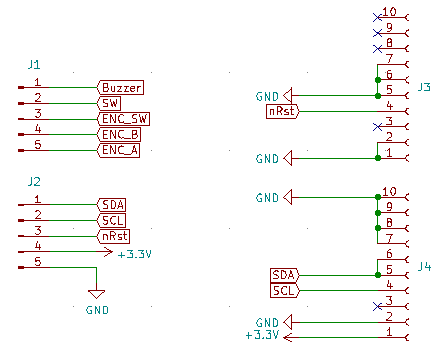
\includegraphics[width=.75\textwidth]{sec6/images/Display_PCB} 
\centering
\captionsetup{width=.95\textwidth}
\caption[Schaltplan des Bedienungs-Boards 1]{Schaltplan des Bedienungs-Boards mit den Stiftleisten J1 und J2 zur Verbindung mit dem Mikrocontroller und den Buchsenleisten J3 und J4 für das Display}\centering
\label{fig:BedienungsBoard1}
\end{figure}

\begin{figure}[H] %H für Positionierung hier
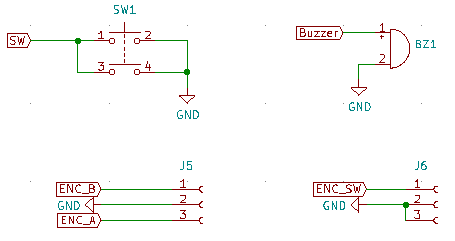
\includegraphics[width=.90\textwidth]{sec6/images/Display_PCB2} 
\centering
\captionsetup{width=.95\textwidth}
\caption[Schaltplan des Bedienungs-Boards 2]{Schaltplan des Bedienungs-Boards mit dem Drehencoder, dem Taster und dem Summer}\centering
\label{fig:BedienungsBoard2}
\end{figure}

\subsection{Programmierung der Steuerelemente}\label{Sec6Sub3}
Die drei Signale des Drehencoders ENC\_A, ENC\_B und ENC\_SW und das Signal SW des Tasters sind als Pulldown-Anschlüsse ausgeführt. Diese Signale werden im Mikrocontroller über einen internen Pull-Widerstand auf \SI{3,3}{\volt} gezogen. Die beiden Signale ENC\_A und ENC\_B liefern zwei um \SI{90}{\degree} verschobene Rechtecksignale, dessen Frequenz sich mit der Drehgeschwindigkeit ändert. Durch den Phasenversatz um \SI{90}{\degree} kann die Drehrichtung bestimmt werden. Dabei wird bei einer Flanke vom Signal \glqq ENC\_A\grqq{} der Spannungspegel vom Signal \glqq ENC\_B \grqq{} bestimmt. Aus der Information, ob es sich um eine fallende oder steigenden Flanke des Signals ENC\_A handelt und ob der Spannungspegel des Signals ENC\_B \SI{3,3}{\volt} oder \SI{0}{\volt} ist, wird die Drehrichtung bestimmt.\vspace{11pt}

Das Signal Buzzer lässt bei anlegen einer Spannung den internen Quarz des Summers mit seiner charakteristischen Frequenz schwingen. Dadurch können Eingaben des Benutzers akustisch bestätigt werden.

\subsubsection{Taster auswerten}\label{sec:Taster}
Im Flussablaufdiagramm in Abbildung \ref{fig:FlussablaufEncTaster} ist zu erkennen, dass beide Taster mit einer Abtastzeit von \SI{10}{\milli\second} eingelesen werden. Da Taster mechanische Bauteile sind, kommt es bei jedem Betätigen zu ungewollten Pegelwechseln, dem sogenannten Prellen. Dies muss verhindert werden, da dadurch ein einzelner Tastendruck als mehrere interpretiert wird. Soll zum Beispiel ein Zähler per Tastendruck inkrementiert werden, wird bei einem prellenden Taster der Zähler pro Druck nicht um einen sondern um mehrere Schritte erhöht. Die Anzahl, um wie viel der Zähler erhöht wird, hängt davon ab, wie viele Pegelwechsel durch das Prellen erzeugt und mit welcher Frequenz der Taster ausgelesen wird. Um das Prellen zu verhindern, wird auf eine Software-Entprellung zurückgegriffen. Dabei wird ein Tastendruck nur erkannt, wenn sich der Spannungspegel des Tasters für vier Abtastzyklen nicht ändert. Dies entspricht bei einer Abtastzeit von \SI{10}{\milli\second} einer Zeit von \SI{40}{\milli\second}. Bei diesem Verfahren ist es wichtig, dass der Taster mindestens die vierfache Zeit der Abtastzeit betätigt wird. Beim Entprellen wird zuerst abgefragt, ob sich der eingelesene Zustand des Tasters zum vorherigen entprellten Zustand geändert hat. Ist dies der Fall wird ein Zähler dekrementiert. Der Zähler zählt dabei von drei bis null. Erreicht dieser den Wert null oder wird ein Zustand eingelesen, der dem zuvor entprelltem Zustand entspricht, wird der Zähler auf den Wert drei zurückgesetzt. Wechselt der Zähler von null auf drei, wird der Tastendruck als solcher erkannt.\vspace{11pt}

\begin{figure}[H]	
\centering
	\begin{tikzpicture}[node distance=1.5cm]
		\node (start) [startstop] {Start};
		\node (prInit) [process, below of=start] {counter = 0};
		\node (EncIn)[io, below of=prInit]{Encoder einlesen};
		\node (prENC) [process, below of=EncIn] {Encoder auswerten};
		\node (decCounter)[decision,below of=prENC,yshift=-0.5cm]{counter$\geq$10?};
		\node (SWIn)[io,below of = decCounter,yshift=-1cm]{Taster einlesen};
		\node (prSW) [process, below of=SWIn] {Taster auswerten};
		\node (prDelay) [process, below of=prSW] {warte \SI{1}{\milli\second}};
		
		
		\draw [arrow] (start) -- (prInit);
		\draw [arrow] (prInit) -- (EncIn);
		\draw [arrow] (EncIn) -- (prENC);
		\draw [arrow] (prENC) -- (decCounter);
		\draw [arrow] (decCounter) -- node[anchor=east]{ja} (SWIn);
		\draw [arrow] (SWIn) -- (prSW);
		\draw [arrow] (prSW) -- (prDelay);
		
		\draw [arrow](decCounter) -- node[anchor = south]{nein} ++(3,0)|-(EncIn);
		\draw [arrow](prDelay) |- ++(3,-1)--+(0,6.5);
				
	\end{tikzpicture}
	
	\caption[Flussablaufdiagramm Taster und Drehencoder einlesen]{Flussablaufdiagramm zum Einlesen des Encoders jede Millisekunde und der Taster alle zehn Millisekunden}
	\label{fig:FlussablaufEncTaster}
\end{figure}

Im C-Code wird der Zähler mit zwei 32 Bit Variablen implementiert. Dabei wird aus jeweils einem Bit der beiden Variablen ein 2bit Zähler gebildet. Dadurch entstehen mit nur zwei Variablen insgesamt 32 Zähler, die von drei bis null zählen können. Dies macht jedoch die Implementierung der Zählfunktion schwieriger, da der Zähler nicht mit einem Postdekrement und if-Abfragen realisiert werden kann. Diese Funktionen müssen durch Bitoperationen ersetzt werden, die die ganze 32 Bit Variable abfragen und ändern können (siehe \cite{Debounce}, Kapitel \glqq Timer-Verfahren (nach Peter Dannegger)\grqq).

\subsubsection{Drehencoder auswerten}\label{sec:Drehencoder}
Im Flussablaufdiagramm in Abbildung \ref{fig:FlussablaufEncTaster} werden die beiden um \SI{90}{\degree} phasenverschobenen Signale des Drehencoders mit einem Zeitabstand von \SI{1}{\milli\second} ausgelesen. Im Anschluss daran müssen daraus die Drehrichtung und die Anzahl der gedrehten Schritte ermittelt werden. Dazu wird in einer Variable der aktuell gemessene und der jeweils letzte Wert der beiden Drehencoderanschlüsse als je ein Bit gespeichert. Dabei liegt in Bit0 der aktuelle Zustand von ENC\_B, in Bit1 der aktuelle Zustand von ENC\_A, in Bit2 der letzte Zustand von ENC\_B und in Bit3 der letzte Zustand von ENC\_A. Die daraus entstehende 4bit-Zahl bildet den Index eines Arrays, welches zeigt, ob der Drehencoder nach links oder nach rechts gedreht worden ist. Steht in der Variable zum Beispiel der Wert 1101\textsubscript{2} (13\textsubscript{10}) bedeutet das, dass die vorherigen Zustände HIGH, der aktuelle Zustand ENC\_A LOW und ENC\_B HIGH sind. Daraus ist abzuleiten, dass eine fallende Flanke des Signals ENC\_A und ein HIGH Pegel am Signal ENC\_B anliegt. In dem Array an der Stelle 13 steht der Wert -1, was eine Drehung im Uhrzeigersinn repräsentiert. Im Falle von 1000\textsubscript{2} (8\textsubscript{10}) liegt eine fallende Flanke an ENC\_A und ein LOW Pegel an ENC\_B an. Daraus ergibt sich im Array der Wert 1 an der Stelle acht, was eine Drehrichtung gegen den Uhrzeigersinn darstellt (siehe \cite{ENC}).
\newpage
\subsection{Programmierung der Anzeige}\label{Sec6Sub2}
Für die Anzeige von Fahrzeugparametern wird ein 64x128 Pixel großes \ac{OLED} verwendet, dessen Ansteuerung über eine \ac{I2C} Schnittstelle erfolgt.  Mit dem Pin6 von Buchsenleiste J3 wird die \ac{I2C} Adresse auf 3C\textsubscript{16} (GND) oder 3E\textsubscript{16} (\SI{3,3}{\volt}) festgelegt. Dem Schaltplan in Abbildung \ref{fig:BedienungsBoard1} ist zu entnehmen, dass die Adresse auf 3C\textsubscript{16} festgelegt ist. Außerdem wird das Reset Signal des Controllers an den Pin4 der Buchsenleiste J3 angelegt.

\subsubsection{Funktionsweise des \acl{OLED}s}\label{sec:FunktionOLED}
Auf der Platine des Displays ist der Displaycontroller SSD1309 von SOLOMON SYSTECH verbaut. Dieser kommuniziert mit dem Mikrocontroller und steuert die Segment- und COM-Anschlüsse des Displays. Das Display besitzt 64 COM-Anschlüsse für die Kathoden der LEDs und 128 Segmentanschlüsse für die Anoden. Jeder COM-Anschluss entspricht einer Zeile des Displays und jeder Segmentanschluss einer Spalte (siehe Schaltplan in Abbildung \ref{fig:OLEDSchaltplan}). Somit kann durch Auswahl einer Reihe mit einem COM-Anschluss und durch ansteuern des Segmentanschlusses jedes Pixel angesprochen werden. Im Displaycontroller ist ein \ac{RAM} mit 64 Zeilen und 128 Spalten verbaut. Jeder Zeile des Speichers ist eine Zeile des Displays (COM-Anschluss) und jeder Spalte des Speichers eine Spalte des Displays (Segmentanschluss) zugeordnet. Somit ist jedem Bit im \ac{RAM} ein Pixel auf dem Display zugewiesen. Acht Zeilen des Speichers werden zu einer Seite zusammengefasst. Dadurch werden acht Zeilen mit einer 8bit großen Variable angesprochen. Bit0 entspricht der ersten Zeile und Bit7 der achten Zeile der Seite. Ein Bild auf dem Display wird aufgebaut indem zuerst das Segment SEG0 mit einem HIGH Pegel ausgewählt wird und die ersten acht im \ac{RAM} gespeicherten Pixelwerte an den Anschlüssen COM0 bis COM7 angelegt werden. Danach wird das Segment SEG1 ausgewählt und die zweiten acht Pixelwerte an die gleichen COM-Anschlüsse angelegt. Dies wird bis zum letzten Segment fortgeführt. Im Anschluss daran wird wieder das Segment SEG0 ausgewählt. Diesmal werden die Pixelwerte jedoch an die Anschlüsse COM8 bis COM15 angelegt. Nachdem das letzte Segment und die letzten acht COM-Anschlüsse angesteuert worden sind, beginnt der Durchlauf von vorne. In den Einstellungen des Displaycontrollers kann eingestellt werden, von welcher Startseite bis zu welcher Stoppseite die COM-Anschlüsse angesteuert werden. Dadurch können Seiten am oberen und unteren Displayrand ausgelassen und somit der Displaybereich vertikal beschränkt werden. Das Start- und Stoppsegment kann ebenfalls bestimmt und somit der rechte und linke Displayrand beschränkt werden. Außerdem kann die horizontale Orientierung festgelegt werden, indem man die Zuordnung des Segments SEG0 auf die Speicherspalte null oder 127 legt. Dadurch werden die ersten Pixelwerte im Speicher nicht in die Spalte des Segments SEG0 sondern in die Spalte von Segment SEG127 geschrieben. Die Einstellung der vertikalen Orientierung erfolgt mit der Richtung, mit der die Zeilen des Speichers auf die COM-Anschlüsse gelegt werden.

\begin{figure}[H]
\begin{circuitikz}
\draw 	(0,0)node[anchor=south]{SEG0}to[short,o-*](0,-1) to[led,-*] (0,-3)
		(2,0)node[anchor=south]{SEG1}to[short,o-*](2,-1) to[led,-*] (2,-3)
		(4,-2)node[circ]{}
		(5,-2)node[circ]{}
		(6,-2)node[circ]{}
		(8,0)node[anchor=south]{SEG127}to[short,o-*](8,-1) to[led] (8,-3)
				
		(1,-3)node[jump crossing](j00){}
		(3,-3)node[jump crossing](j10){}
		
		(-1,-3)node[anchor=east]{COM0}to[short,o-](j00.west) 
		(j00.east)--(j10.west)
		(j10.east)--(3.5,-3)
		(7.5,-3)--(8,-3)

		(0,-4)to[led,-*] (0,-6) (0,-1)-|(j00.north)(j00.south)to[short,-*](1,-4)--(0,-4)
		(2,-4)to[led,-*] (2,-6)	(2,-1)-|(j10.north)(j10.south)to[short,-*](3,-4)--(2,-4)
		(4,-5)node[circ]{}
		(5,-5)node[circ]{}
		(6,-5)node[circ]{}
		(8,-4)to[led] (8,-6)	(8,-1)--(9,-1)to[short,-*](9,-4)--(8,-4)
		
		(1,-6)node[jump crossing](j01){}
		(3,-6)node[jump crossing](j11){}		
			
		(-1,-6)node[anchor=east]{COM1}to[short,o-](j01.west) 
		(j01.east)--(j11.west)
		(j11.east)--(3.5,-6)
		(7.5,-6)--(8,-6)
		
		(1,-4)--(j01.north)	(j01.south)--(1,-6.5)
		(3,-4)--(j11.north)	(j11.south)--(3,-6.5)
		(9,-4)--(9,-6.5)
		
		
		(0,-7)node[circ]{}
		(0,-7.5)node[circ]{}
		(0,-8)node[circ]{}
		
		(2,-7)node[circ]{}
		(2,-7.5)node[circ]{}
		(2,-8)node[circ]{}
		
		(8,-7)node[circ]{}
		(8,-7.5)node[circ]{}
		(8,-8)node[circ]{}
		
		
		(0,-9)to[led,-*] (0,-11) 	%(0,-1)-|(j00.north)(j00.south)to[short,-*](1,-4)--(0,-4)
		(2,-9)to[led,-*] (2,-11)	%(2,-1)-|(j10.north)(j10.south)to[short,-*](3,-4)--(2,-4)
		(4,-10)node[circ]{}
		(5,-10)node[circ]{}
		(6,-10)node[circ]{}
		(8,-9)to[led] (8,-11)		%(8,-1)--(9,-1)to[short,-*](9,-4)--(8,-4)
		
	
		
		(-1,-11)node[anchor=east]{COM63}to[short,o-](3.5,-11)(7.5,-11)--(8,-11)
		(0,-9)-|(1,-8.5)
		(2,-9)-|(3,-8.5)
		(8,-9)-|(9,-8.5)	
;

\draw[dotted]
	(3.5,-3)--(7.5,-3)
	(3.5,-6)--(7.5,-6)
	(3.5,-11)--(7.5,-11)

	(1,-6.5)--(1,-8.5)
	(3,-6.5)--(3,-8.5)
	(9,-6.5)--(9,-8.5)
;
\end{circuitikz}
\caption[Schaltplan OLED]{Repräsentativer Schaltplan des \acp{OLED} mit Segment- und COM-Anschlüssen}
\label{fig:OLEDSchaltplan}
\end{figure}

\subsubsection{I2C Ansteuerung}\label{sec:OLEDI2C}
%i2c_rtos_interface.c
%ssd1309.c
%ssd1309_rtos.c

Die Kommunikation mit dem \ac{OLED} erfolgt mit einer \ac{I2C} Schnittstelle. Dazu wird auf dem Mikrocontroller ein sogenanntes Flexcomm Modul verwendet. Dieses Modul beinhaltet mehrere Schnittstellen wie zum Beispiel \ac{UART} oder \ac{I2C}. Zu Beginn wird der Port-Pin P3.24 als SCL und der Port-Pin P3.25 als SDA des Flexcomm2 Moduls konfiguriert. Danach wird das Modul mit der Funktion \glqq I2C\_MasterInit\grqq{} von NXP so initialisiert, dass die Taktfrequenz des SDA Signals \SI{400}{\kilo\hertz} beträgt. Dabei ergibt sich Problem, dass das Modul zunächst keine Daten sendet. Nach dem Debuggen und Überprüfen jedes Registers des Moduls wird festgestellt, dass der Takt für das Modul deaktiviert ist. Ärgerlich ist das, da bei der Konfiguration auf Funktionen zurückgegriffen wird, die von NXP entwickelt worden sind und funktionieren sollten. Nachdem der Takt (\SI{12}{\mega\hertz}) für das Flexcomm2 Modul aktiviert ist, werden die Daten wie gewünscht über die Schnittstelle gesendet. Jedoch beträgt die von der Initialisierungsfunktion eingestellte Taktfrequenz statt der angegebenen \SI{400}{\kilo\hertz} nur \SI{333}{\kilo\hertz}. Um den Fehler zu finden, wird in den Registern überprüft, welche Werte für die Erzeugung der Taktfrequenz verwendet werden. Zur Erzeugung wird die Taktfrequenz des Flexcomm2 Moduls mit einem Teiler erniedrigt. Mit zwei Werten werden für die HIGH und LOW Zeiten die Anzahl der Takte (Flexcomm-Takt) angegeben. Nach der Initialisierungsfunktion wird ein Teiler von drei und eine HIGH und LOW Zeit von 5 Takten festgelegt. Die Taktfrequenz berechnet sich über Gleichung \ref{eq:I2CTakt}. Setzt man darin die Werte der Register ein, ergibt sich die gewollte Frequenz von \SI{400}{\kilo\hertz}.

\begin{equation}\label{eq:I2CTakt}
\frac{f_{flexcomm}}{DIV_{CLK}\cdot\left(t_{cyc_{HIGH}}+t_{cyc_{LOW}}\right)}
\end{equation}

Im Datenblatt des Mikrocontrollers sind Werte angegeben, mit denen, bei einer Flexcomm-Taktfrequenz von \SI{12}{\mega\hertz}, eine Taktfrequenz der \ac{I2C}-Schnittstelle von \SI{400}{\kilo\hertz} erzeugt wird. Dabei wird ein Teiler von sechs, eine HIGH Zeit von zwei und eine LOW Zeit von drei Taktzyklen verwendet (vgl. \cite{Semic} Seite 462, Tabelle 496). Mit der Gleichung \ref{eq:I2CTakt} berechnet sich die Taktfrequenz der Schnittstelle zu \SI{400}{\kilo\hertz}. Die drei richtigen Werte werden nach der Initialisierungsfunktion per Hand in den Registern gesetzt.\vspace{11pt}

Um den Prozessor zu entlasten, wird auf die zu sendenden Daten per \ac{DMA} zugegriffen. Dadurch werden diese parallel zum Prozessor in das Senderegister des Flexcomm2 Moduls geladen und der Prozessor hält sich nicht mit hin- und herschieben von Daten auf. Zuallererst wird das \ac{DMA} Modul DMA0 mit der von NXP zur Verfügung gestellten Funktion \glqq DMA\_Init\grqq{} initialisiert. Dem Datenblatt wird in Tabelle 300 entnommen, dass der Kanal 5 mit der \ac{I2C} Funktion des Flexcomm2 Moduls verbunden ist. Deshalb wird mit der ebenfalls bereitgestellten Funktion \glqq DMA\_EnableChannel \grqq{} der Kanal 5 freigegeben. Im Anschluss daran wird mit den beiden Funktionen \glqq DMA\_CreateHandle\grqq{} und \glqq I2C\_MasterTransferCreateHandleDMA\grqq{} die Funktionalität des \ac{DMA}s mit dem Flexcomm2 Modul freigegeben.\vspace{11pt}

Mit der Funktion \glqq I2C\_MasterTransferNonBlocking\grqq{} wird eine Übertragung über \ac{I2C} und \ac{DMA} begonnen. Dieser Funktion wird in einer Variable ein Pointer auf die zu sendende Variable und deren Länge übergeben. Sollen anzuzeigende Daten an das \ac{OLED} übertragen werden wird der Funktion ein Pointer auf einen zuvor definierten Displaypuffer und dessen Länge übergeben. Soll eine Konfiguration gesendet werden, muss der Funktion ein Pointer auf eine 8bit Variable und die Länge eins übergeben werden. Die Übergabe in die Funktion erfolgt mit einer \glqq struct\grqq{} Variable, die neben dem Pointer und der Länge noch die Slaveadressse des Displays, eine Variable für die Richtung der Übertragung (schreiben oder lesen) und eine Variable enthält, die angibt, wie die Start- und Stoppbits gesendet werden. Die Auswahl, ob es sich bei den gesendeten Daten um Konfigurations- oder Anzeigedaten handelt, erfolgt über die sogenannte Subadresse. Diese wird im Anschluss an die Slaveadresse übertragen. Deshalb muss der Funktion ebenfalls die Subadresse und deren Länge übergeben werden.

\subsubsection{Konfiguration des Displays}
Zu Beginn werden einige Resetparameter (siehe Tabelle \ref{tab:InitOLED}) übertragen, die das Display zuerst ausschalten und den Kontrast einstellen. Danach wird ein Kommando gesendet, das den Speicher des \ac{OLED} Controllers so einstellt, dass dessen Inhalt direkt auf dem Display angezeigt wird. Eine andere Möglichkeit ist es, den Inhalt des \ac{RAM}s zu ignorieren. Das Display wird im Standard-Modus (Normal Mode) gestartet. Dies bedeutet, dass eine 1 im Speicher die Pixel-LED einschaltet. Wird der horizontale Modus konfiguriert, wie es in dieser Anwendung der Fall ist, wird das Bild, das auf dem Display angezeigt werden soll, wie im Kapitel \ref{sec:FunktionOLED} beschrieben ist, aufgebaut. Der Befehl 40\textsubscript{16} bestimmt die Zeile des Displays, welche dem Anschluss COM0 zugewiesen wird. Durch Ändern dieses Wertes kann der Inhalt des Displays nach oben bzw. unten geschoben werden. Mit dem nächsten Kommando wird die horizontale Orientierung eingestellt. In diesem Fall wird der Inhalt des Speichers von Segment SEG127 nach SEG0 ausgegeben. Mit dem Befehl \glqq scan from COM N-1 to COM0\grqq{} wird die vertikale Orientierung festgelegt, wobei N dem \glqq MUX ratio\grqq{} (Anzahl der COM-Anschlüsse) entspricht. Die Hardware der COM Pins wird auf ihren Reset Wert eingestellt, was bedeutet, dass die geraden Zeilen mit den ersten 32 COM-Anschlüssen und die ungeraden mit den restlichen 32 COM-Anschlüssen verbunden sind. Danach werden die GPIO Pins als Eingänge konfiguriert. Das nächste Kommando stellt die Frequenz des Displays auf ihren korrekten Wert. Außerdem wird die Anzahl der Takte in Phase 1 und 2 auf jeweils zwei Takte gesetzt. In Phase 1 wird das Pixel ent- und in Phase 2 auf ihren neuen Wert aufgeladen. Diese Werte müssen den Kapazitätswerten der Pixel angepasst werden. Das letzte Kommando stellt die Spannung, bezogen auf die Versorgungsspannung des Displays, ein, wenn die COM-Anschlüsse deaktiviert sind. Alle Konfigurationseinstellungen sind im Datenblatt des Display Controllers zu finden (vgl \cite{SSD1309}).\vspace{11pt}

Nach der Konfiguration des Resets erfolgt die Konfiguration, welche für die Anwendung auf dem Fahrzeug passend ist. Dazu wird die horizontale Orientierung so eingestellt, dass die Spaltenadresse 127 im Speicher dem Segment SEG127 entspricht. Ebenso wird die vertikale Orientierung auf einen Wert festgelegt, sodass das Display von den COM-Anschlüssen COM0 nach COM64 angesteuert wird. Am Ende wird das Display eingeschaltet und ist einsatzbereit.

\begin{table}[H]
\centering
	\begin{tabular}{|c|l||c|l|}
	\hline
	AE&Display off&A8&set MUX ratio to\\
	&&3F&64MUX\\
	\hline
	81&Contrast Controll&C8&scan from COM N-1\\
	7F&&&to COM 0\\
	\hline
	A4&display on, output RAM content&D3&no vertical shift\\
	&&00&\\
	\hline
	A6&Normal display mode&DA&set COM pins\\
	&&12&hardware to reset\\
	\hline
	20&Horizontal mode&DC&GPIO pins are inputs\\
	00&&02&\\
	\hline
	21&set column address&D5&increace F\textsubscript{OSC} frequency\\
	00&start address&F0&\\
	7F&end address&&\\
	\hline
	22&set page address&D9&Phase 1 and 2 period to reset\\
	00&to reset value&22&\\
	07&&&\\
	\hline
	40&set display start&DB&set V\textsubscript{COMH} to $0.78 \cdot V_{cc}$\\
	&line to top line&34&\\
	\hline
	A1&column address 127&&\\
	&is SEG0&&\\
	\hline
	\end{tabular}
	\caption[Initialisierungswert \ac{OLED}]{Werte, die der Reihe nach über \ac{I2C} zum \ac{OLED} gesendet werden}
	\label{tab:InitOLED}
\end{table}


\subsection{Darstellungen auf dem \acl{OLED}}\label{sec:OLEDDarstellen}
Die im Folgenden vorgestellten Funktionen werden zur Darstellung von Formen, Text und Zahlen verwendet. Beim Aufruf einer dieser Funktionen wird eine Variable gesetzt, welche anzeigt, dass dem \ac{OLED} neue Daten gesendet werden müssen. In einem Echtzeittask wird diese Variable alle \SI{30}{\milli\second} geprüft und, wenn notwendig, die neuen Daten gesendet und dargestellt. Die Daten werden in einer globalen Variable, dem Displaypuffer \glqq s\_disp\_0\_buffer\grqq{}, gespeichert.

\subsubsection{Pixelansteuerung}\label{sec:OLEDPixel}
Mit der Funktion \glqq ssd1309\_set\_pixel\grqq{} wird ein Pixel an einer vorgegebenen Position, also das anzusprechende Bit im Displaypuffer, gesetzt oder gelöscht.

\subsubsection{Rechteck zeichnen}\label{sec:OLEDRect}
Zur Darstellung von Rechtecken wird die Funktion \glqq ssd1309\_draw\_rect\grqq{} verwendet. Dieser werden die Koordinaten der linken oberen und rechten unteren Ecke und eine Variable übergeben, die festlegt, ob das Rechteck ausgefüllt ist oder nur die Begrenzungslinie angezeigt werden soll. Außerdem muss angegeben werden, ob die Pixel des Rechtecks gesetzt oder gelöscht werden sollen. In der Funktion werden mit zwei Schleifen alle Pixel innerhalb des Rechtecks durchlaufen und für jedes Pixel bestimmt, ob dieses angezeigt werden soll oder nicht. Jedes Pixel wird mit der Funktion \glqq ssd13099\_set\_pixel\grqq{} aus Kapitel \ref{sec:OLEDPixel} im Displaypuffer gesetzt oder gelöscht.

\subsubsection{Buchstabe darstellen}\label{sec:OLEDBuchstabe}
Der Funktion \glqq ssd1309\_write\_char\grqq{} wird eine char Variable übergeben, welche am Display angezeigt werden soll. In \glqq struct\grqq -Variablen mit dem Namen \glqq ssd1309\_font\_t\grqq{} sind für alle darstellbaren Buchstaben und Zeichen Werte hinterlegt, die diese in unterschiedlichen Größen darstellen. In der Funktion selbst wird zu Beginn überprüft, ob das übergebene Zeichen ein darstellbares Ascii-Zeichen ist. Ist dies der Fall, muss abgefragt werden, ob das Zeichen innerhalb des Displays liegt. Wenn ja, wird mit zwei Schleifen für jedes Pixel innerhalb der Höhe und Breite des Zeichens überprüft, ob dieses angezeigt werden soll oder nicht. Pixel, die angezeigt werden, werden mit der Funktion \glqq ssd1309\_set\_pixel\grqq{} aus Kapitel \ref{sec:OLEDPixel} angesprochen. Die Position des Zeichens wird über einen Cursor eingestellt, der vor dem Funktionsaufruf gesetzt werden muss. Nachdem die einzelnen Pixel des Zeichens im Displaypuffer gesetzt bzw. gelöscht worden sind, wird der Cursor automatisch inkrementiert.

\subsubsection{Text darstellen}\label{sec:OLEDText}
Die Funktion \glqq ssd1309\_write\_str\grqq{} stellt am Display einen Text dar, der über einen Pointer auf ein Zeichenarray übergeben wird. Dazu wird die in Kapitel \ref{sec:OLEDBuchstabe} beschriebene Funktion für jedes im Text enthaltene Zeichen ausgeführt. Die Position des Textes wird, wie bei den Buchstaben, über den Cursor eingestellt, welcher vor dem Funktionsaufruf gesetzt werden muss.

\subsubsection{Bilder darstellen}\label{sec:OLEDBild}
Die Funktion \glqq ssd1309\_draw\_img\grqq{} stellt Bilder dar, die als Hexadezimalwert abgespeichert sind. Die Position der linken oberen Ecke muss der Funktion übergeben werden. Das Bild wird in einer \glqq struct\grqq{}-Variable mit dem Namen \glqq ssd1309\_img\_t\grqq{} übergeben, die die Breite und Höhe des Bildes enthält. Ausgegeben wird das Bild mithilfe zweier Schleifen, die für jedes Pixel des Bildes überprüfen, ob dieses angezeigt werden soll oder nicht. Dargestellt werden die einzelnen Pixel mit der Funktion \glqq ssd1309\_set\_pixel\grqq{} aus Kapitel \ref{sec:OLEDPixel}.

\subsection{Menüführung}\label{sec:OLEDMenu}
Auf die einzelnen Parameter und Funktionen des Fahrzeugs wird mit verschiedenen Menüs zugegriffen. Zuallererst wird das Hauptmenü aufgerufen. Darin sind die einzelnen Funktionen in unterschiedliche Menüpunkte aufgeteilt. Der Mikrocontroller nimmt die Menüführung auf Basis der Werte des Drehencoders und der beiden Taster vor. Ein Zustandsautomat entscheidet je nach Bedienung, ob der Hauptbildschirm oder ein Menü angezeigt werden soll. Bevor der Zustandsautomat ausgeführt wird, werden die beiden Zustände der entprellten Taster sowie die Anzahl der Schritte gespeichert, die der Drehencoder in eine bestimmte Richtung getätigt hat. Der Zustandsautomat bestimmt das aktuelle, anzuzeigende Menü und ändert den Displaypuffer so ab, dass dieses dargestellt wird.\vspace{11pt}

\textbf{Es gibt insgesamt vier verschieden Arten von Menüs:}
\begin{itemize}
\item MENU\_LINK
\item MENU\_CHECK
\item MENU\_PAGE
\item MENU\_VALUE
\end{itemize}

Jedes Menü besitzt eine \glqq struct\grqq{}-Variable, in der immer die drei gleichen Eigenschaften enthalten sind; die Bezeichnung, die auf dem \ac{OLED} angezeigt wird, die Menüart und eine Kennzeichnung, ob das Menü angeklickt werden kann oder nicht. Ist das angeklickte Menü ein MENU\_LINK, so öffnet sich das ebenfalls in der \glqq struct\grqq{}-Variable enthaltene Folge-Menü. Ist es von der Art MENU\_CHECK, wird mit einem Klick auf dieses eine, in der \glqq struct\grqq{}-Variable als Pointer gespeicherte, Variable inkrementiert. Durch eine spätere, binäre UND-Operation mit 1, erhält man eine Variable, die bei einem Klick aktiviert bzw. deaktiviert wird (01\textsubscript{2} \& 1 = 1; 10\textsubscript{2} \& 1 = 0). Mit der Betätigung eines Menüs der Art MENU\_PAGE, wird eine darin verlinkte Funktion ausgeführt. Wird ein Menü der Sorte MENU\_VALUE betätigt, wird der Wert einer in der \glqq struct\grqq{}-Variable als Pointer verknüpften Variable mit dem Drehencoder erhöht oder erniedrigt. Außerdem wird eine Funktion aufgerufen, wenn sich der Wert dieser Variable verändert. Dies wird zum Beispiel bei der Einstellung der maximalen und minimalen Drehzahl der \acp{BLDCMot} verwendet, um den Wert in das Register des jeweiligen Timer Match Registers zu schreiben. Somit kann z.B. die Einstellung der Drehzahlwerte überprüft werden.

\subsection{Aufbau des \aclp{HMI}}
Das \ac{HMI} wird in einem eigenen Task aufgebaut. Beim ersten Durchlauf wird zuallererst das \ac{OLED} sowie die benötigten Menüs initialisiert. Danach werden im Abstand von einer Sekunde zuerst das Logo von \ac{NXP} und danach das Logo der HAW Landshut angezeigt. Nach wiederum einer Sekunde wird der Hauptbildschirm geöffnet. Dort kann mit dem Taster in das Hauptmenü gewechselt und zwischen dem Drive-, Hardware-, Expert-, About- und Hide Menü gewählt werden. Aus zeitlichen Gründen sind nur das Hardware und Hide Menü implementiert. Das Hide Menü wechselt lediglich vom Hauptmenü zurück auf den Hauptbildschirm.\vspace{11pt} 

Das Hardware Menü enthält Untermenüs für die Kamera, die Motoren und den Summer. Die Menüs für die Kamera und den Summer sind noch nicht implementiert. Mit einem Klick auf Motoren wird in das Motorenmenü gewechselt, in dem die beiden \acp{BLDCMot} sowie der Servo-Motor enthalten sind. Im Servo Menü wird in der ersten Zeile der Port und Pin angezeigt, an welchem das \ac{PWM}-Signal für die Servo-Lenkung ausgegeben wird. In der zweiten Zeile befindet sich ein Menü zum Testen der Lenkwinkel. Dabei wird ein Wert zwischen -100 und 100 mit einer Schrittweite von 1 vom Drehencoder eingestellt. Der Servo lenkt beim Wert -100 auf den vollen Linkseinschlag und beim Wert 100 auf den vollen Rechtseinschlag ein. Im nächsten Menüeintrag wird mit dem Drehencoder der Initialisierungswert, also die Mittelstellung, eingestellt. Dieser Wert wird nach dem Einschalten des Mikrocontrollers angesteuert. Mit den letzten beiden Einträgen wird der linke bzw. rechte, maximale Lenkeinschlag bestimmt.\vspace{11pt}

Wählt man im Motor Menü einen der beiden Antriebe aus, gelangt man in das Menü für den jeweiligen \ac{BLDCMot}. Der erste Menüeintrag zeigt, wie beim Servo Menü, lediglich den Port-Pin des ausgewählten Motors an. Ebenso wie beim Servo ist bei den \ac{BLDCMot} Menüs ein Testmenü enthalten, mit welchem man eine Drehzahl zwischen 0 und 100 vorgeben kann. Die letzten beiden Untermenüs stellen die obere und untere Drehzahl ein.\vspace{11pt}

Jedes Menü enthält als letzten Eintrag ein Untermenü, mit welchem ins jeweils vorangegangene Menü gewechselt werden kann. Ein Klick auf den Taster lässt das \ac{OLED} zum Hauptbildschirm zurückspringen.

\subsection{Anleitung zum Hinzufügen eines neuen Menüs}\label{sec:MenüHinzufügen}

\begin{enumerate}
\item Hinzufügen eines Eintrags in dem Menü, in dem das neue Menü aufgerufen werden soll (\glqq menu\_data.c\grqq)
\item Erhöhen der Anzahl der Einträge um eins (\glqq menu\_data.c\grqq)
\item Erstellen einer Funktion, welche das neue Menü aufruft (\glqq screen.c\grqq{})
\item Erstellen einer Liste mit allen im neuen Menü enthaltenen Untermenüs sowie eines neuen Handlers (\glqq menu\_data.c\grqq)
\item Deklarieren der notwendige Variablen und Funktionen für die neuen Untermenüs (\glqq menu\_data.c\grqq)
\item Initialisieren des neuen Menüs (\glqq hmi.c\grqq)
\end{enumerate}

Soll zum Beispiel im Hardware Menü ein neues Untermenü mit dem Namen \glqq new menu\grqq{} hinzugefügt werden, so muss dafür ein neuer Eintrag (Abbildung \ref{fig:AddMenu1}, roter Rahmen) im Hardwaremenü erstellt werden. Außerdem muss die Variable \glqq entry\_count\grqq{} im zugehörigen \glqq menu\_rtos\_handle\_t\grqq{} inkrementiert werden (siehe Abbildung \ref{fig:AddMenu2}). Im Anschluss daran muss eine Funktion implementiert werden, welche das neue Menü öffnet. Diese ersetzt nur das aktuelle Menü durch das neue Menü (siehe Abbildung \ref{fig:AddMenuFunktion}).

\begin{figure}[H] %H für Positionierung hier
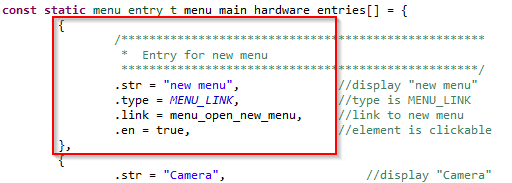
\includegraphics[width=.75\textwidth]{sec6/images/AddMenu1} 
\centering
\captionsetup{width=.95\textwidth}
\caption[Schritt 1: Erstellen eines neuen Menüeintrags]{Schritt 1: Erstellen eines neuen Menüeintrags durch Hinzufügen der im roten Rahmen dargestellten Code-Zeilen}\centering
\label{fig:AddMenu1}
\end{figure}
\begin{figure}[H] %H für Positionierung hier
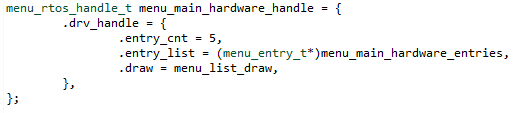
\includegraphics[width=.75\textwidth]{sec6/images/AddMenu2} 
\centering
\captionsetup{width=.95\textwidth}
\caption[Schritt 2: Erhöhen der Anzahl der Menüeinträge um eins]{Schritt 2: Erhöhen der Anzahl der Menüeinträge um eins (entry\_cnt)}\centering
\label{fig:AddMenu2}
\end{figure}
\begin{figure}[H] %H für Positionierung hier
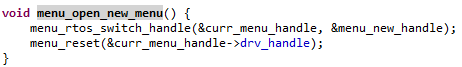
\includegraphics[width=.75\textwidth]{sec6/images/AddMenuFunktion} 
\centering
\captionsetup{width=.95\textwidth}
\caption[Schritt 3: Erstellen einer Funktion zum Menüaufruf]{Schritt 3: Erstellen einer Funktion zum Menüaufruf}\centering
\label{fig:AddMenuFunktion}
\end{figure}

Außerdem müssen in der Datei \glqq menu\_data.c\grqq{} die Einträge des neuen Menüs definiert werden (Schritt 4). Dazu wird zuallererst eine Liste für die Einträge erstellt. Das erste Untermenü mit dem Namen \glqq new1\grqq{} öffnet in diesem Beispiel den Hauptbildschirm. Das zweite Menü \glqq new2\grqq{} aktiviert bzw. deaktiviert die Variable \glqq variableCheck\grqq{}. Mit dem Menü \glqq new3\grqq{} wird die Variable \glqq variableValue\grqq{} mit dem Drehencoder verändert und die Funktion \glqq func\_value\grqq{} ausgeführt. Das letzte Menü mit dem Namen \glqq new4\grqq{} führt die Funktion \glqq func\_page\grqq{} aus, welche den kompletten Bildschirm füllt (alle Pixel-LEDs ein). Außerdem muss in diesem Schritt der Handler definiert werden, der die eben erstellte Liste mit den Einträgen, deren Anzahl sowie die bereits vorhandene Funktion zum Darstellen der Untermenüs enthält. Wichtig ist, dass der Handler in der Datei \glqq menu\_data.h\grqq{} bekannt ist. Nur so kann in der Datei \glqq screen.c\grqq{} das neue Menü geöffnet werden (siehe Abbildung \ref{fig:AddMenuPrototyp}).

\begin{figure}[H] %H für Positionierung hier
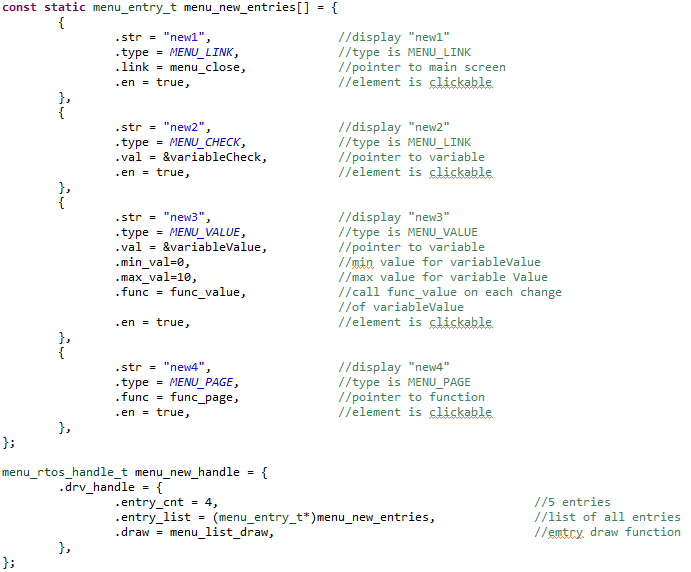
\includegraphics[width=.75\textwidth]{sec6/images/AddMenu3} 
\centering
\captionsetup{width=.95\textwidth}
\caption[Schritt 4.1: Liste mit Einträgen des neuen Menüs erstellen]{Schritt 4.1: Liste mit Einträgen des neuen Menüs erstellen}\centering
\label{fig:AddMenu3}
\end{figure}
\begin{figure}[H] %H für Positionierung hier
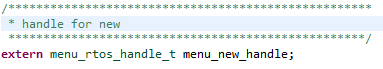
\includegraphics[width=.75\textwidth]{sec6/images/AddMenuPrototyp} 
\centering
\captionsetup{width=.95\textwidth}
\caption[Schritt 4.2: Hinzufügen des Menü Handlers im Header]{Schritt 4.2: Hinzufügen des Menü Handlers im Header (\glqq menu\_dat.h\grqq{})}\centering
\label{fig:AddMenuPrototyp}
\end{figure}


Die Funktion \glqq func\_page\grqq{} (siehe Abbildung \ref{fig:PageFunction}) wird in der Datei \glqq screen.c\grqq{} angegeben (Schritt 5). Diese nimmt den Semaphor des Display, setzt jedes Bit im Displaypuffer, bis auf die Kopfzeile der Anzeige, und gibt den Semaphor wieder frei.

\begin{figure}[H] %H für Positionierung hier
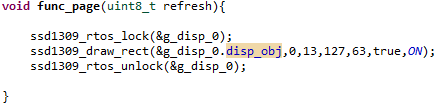
\includegraphics[width=.75\textwidth]{sec6/images/PageFunction} 
\centering
\captionsetup{width=.95\textwidth}
\caption[Schritt 5: Deklarieren der notwendige Variablen und Funktionen für die neuen Untermenüs]{Schritt 5: Deklarieren der notwendige Variablen und Funktionen für die neuen Untermenüs}\centering
\label{fig:PageFunction}
\end{figure}

Nach der Initialisierung des neuen Menüs (Schritt 6) kann dieses aufgerufen werden. Das neu erzeugte Menü ist in Abbildung \ref{fig:NewMenu} und der mit der Funktion \glqq func\_page\grqq{} voll gefüllte Bildschirm in Abbildung \ref{fig:funcPage} dargestellt.

\begin{figure}[H] %H für Positionierung hier
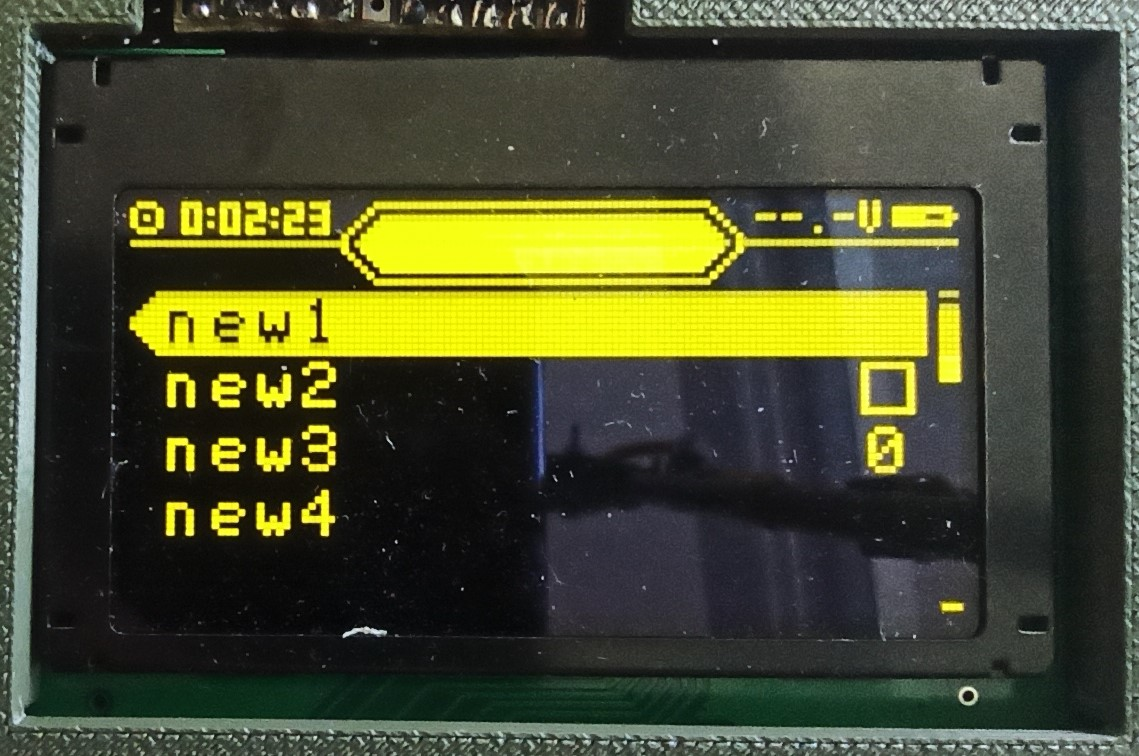
\includegraphics[width=.75\textwidth]{sec6/images/NewMenu} 
\centering
\captionsetup{width=.95\textwidth}
\caption[Anzeige des neu erstellten Menüs auf dem \ac{OLED}ü]{Anzeige des neu erstellten Menüs auf dem \ac{OLED}}\centering
\label{fig:NewMenu}
\end{figure}
\begin{figure}[H] %H für Positionierung hier
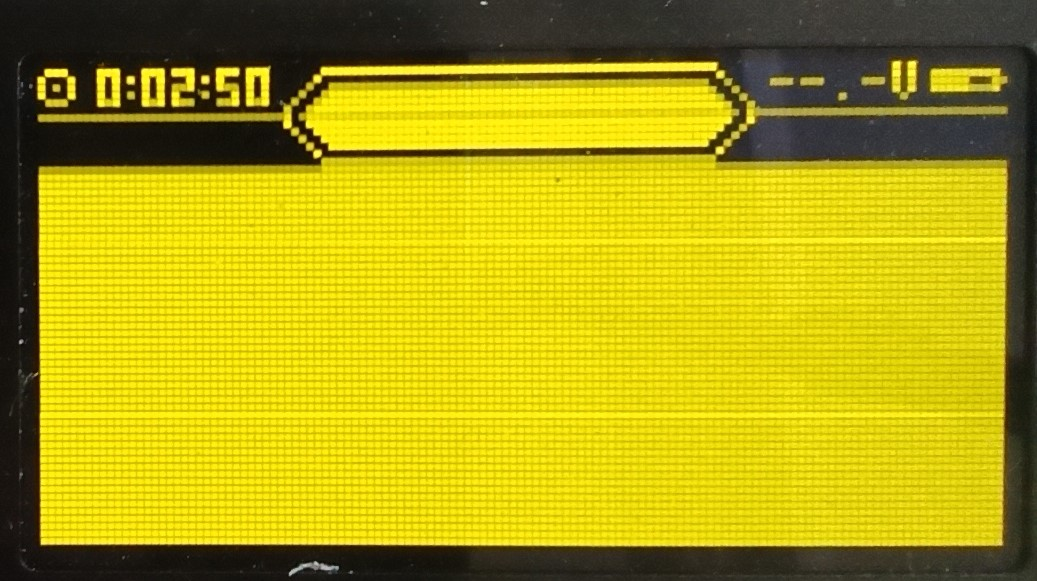
\includegraphics[width=.75\textwidth]{sec6/images/funcPage} 
\centering
\captionsetup{width=.95\textwidth}
\caption[Mit der Funktion \glqq func\_Page\grqq{} erzeugter, voll gefüllter Bildschirm]{Mit der Funktion \glqq func\_Page\grqq{} erzeugter, voll gefüllter Bildschirm}\centering
\label{fig:funcPage}
\end{figure}

\subsection{Verwendung des \aclp{EEPROM}}\label{sec:EEPROM}
Die Fahrzeugparameter, die mit dem \ac{OLED} eingestellt werden können, sollen auch nach der Trennung von der Versorgungsspannung erhalten bleiben. Deshalb werden diese in das Controller-eigene \ac{EEPROM} gespeichert.\vspace{11pt}

Das \ac{EEPROM} wird gleich nach dem Start des Mikrocontrollers mit der Funktion \glqq EEPROM\_Init\grqq{} initialisiert. Danach werden die im \ac{EEPROM} gespeicherten Werte  mit der \glqq memcpy\grqq -Funktion in ein Array mit allen Parametern kopiert. Diese Funktion kopiert einen ganzen Speicherbereich mit einer vorgegebenen Länge ab einer Startadresse an eine andere Adresse. Sollen Daten ins \ac{EEPROM} gespeichert werden, wird zuerst das Array mit den Parametern mit der \glqq memcpy\grqq -Funktion in den Speicherbereich des \acp{EEPROM} geschrieben. Danach müssen diese mit der Funktion \glqq EEPROM\_WritePage\grqq{} fest in den Speicher geschoben werden. Die Daten werden automatisch gespeichert, wenn von einem Menü in den Hauptbildschirm gewechselt wird. Im Hardwaremenü gibt es einen Eintrag \glqq Restore def.\grqq , mit dem die Parameter auf deren Ursprungswerte zurückgesetzt werden können.

\subsection{Ausblick zur Programmierung des Displays}\label{sec:DispAusblick}
Eine sinnvolle Funktionsweise, die mit dem \ac{OLED} relativ einfach realisierbar ist, ist die Anzeige der Daten, die die Kamera liefert (näheres dazu in Kapitel \ref{Sec7Sub3} \glqq{}\nameref{Sec7Sub3}\grqq{}). Dazu kann die Menüart \glqq MENU\_PAGE\grqq{} verwendet werden. Die Anzahl der Kamerapixel stimmt zufälligerweise mit der Anzahl der Pixel auf dem Display überein. In der Funktion des \glqq MENU\_PAGE\grqq -Menüs, kann für jeden Kamerapixel ein Displaypixel mit unterschiedlicher Höhe verwendet werden. Die Höhe kann dabei dem Wert entsprechen, den die Kamera für diesen Pixel liefert.
\newpage